%%%%%%%%%%%%%%%%%%%%%%%%%%%%%%%%%%%%%%%%%
% Journal Article
% LaTeX Template
% Version 1.3 (9/9/13)
%
% This template has been downloaded from:
% http://www.LaTeXTemplates.com
%
% Original author:
% Frits Wenneker (http://www.howtotex.com)
%
% License:
% CC BY-NC-SA 3.0 (http://creativecommons.org/licenses/by-nc-sa/3.0/)
%
%%%%%%%%%%%%%%%%%%%%%%%%%%%%%%%%%%%%%%%%%

%----------------------------------------------------------------------------------------
%	PACKAGES AND OTHER DOCUMENT CONFIGURATIONS
%----------------------------------------------------------------------------------------

\documentclass[11pt]{article}

\usepackage[sc]{mathpazo} % Use the Palatino font
\usepackage[utf8]{inputenc}
\usepackage[T1]{fontenc} % Use 8-bit encoding that has 256 glyphs
\linespread{1.05} % Line spacing - Palatino needs more space between lines
\usepackage{microtype} % Slightly tweak font spacing for aesthetics

%\usepackage[hmarginratio=1:1,top=32mm]{geometry} % Document margins
%\usepackage{multicol} % Used for the two-column layout of the document
\usepackage[hang, small,labelfont=bf,up,textfont=it,up]{caption} % Custom captions under/above floats in tables or figures
\usepackage{booktabs} % Horizontal rules in tables
\usepackage{float} % Required for tables and figures in the multi-column environment - they need to be placed in specific locations with the [H] (e.g. \begin{table}[H])
\usepackage[hidelinks]{hyperref} % For hyperlinks in the PDF

\usepackage{lettrine} % The lettrine is the first enlarged letter at the beginning of the text
%\usepackage{paralist} % Used for the compactitem environment which makes bullet points with less space between them

\usepackage{todonotes}
\usepackage{graphicx}
\usepackage{amsmath,amssymb,amsfonts}
\usepackage{subcaption}
\providecommand{\abs}[1]{\left \lvert #1 \right \rvert}

\usepackage{abstract} % Allows abstract customization
\renewcommand{\abstractnamefont}{\normalfont\bfseries} % Set the "Abstract" text to bold
\renewcommand{\abstracttextfont}{\normalfont\small\itshape} % Set the abstract itself to small italic text

\usepackage{titlesec} % Allows customization of titles
%\renewcommand\thesection{\Roman{section}} % Roman numerals for the sections
%\renewcommand\thesubsection{\Roman{subsection}} % Roman numerals for subsections
\titleformat{\section}[block]{\large\scshape\centering}{\thesection.}{1em}{} % Change the look of the section titles
\titleformat{\subsection}[block]{\large}{\thesubsection.}{1em}{} % Change the look of the section titles

\usepackage{fancyhdr} % Headers and footers
\pagestyle{fancy} % All pages have headers and footers
\fancyhead{} % Blank out the default header
\fancyfoot{} % Blank out the default footer
%\fancyhead[C]{Running title $\bullet$ November 2012 $\bullet$ Vol. XXI, No. 1} % Custom header text
\fancyfoot[RO,LE]{\thepage} % Custom footer text

%----------------------------------------------------------------------------------------
%	TITLE SECTION
%----------------------------------------------------------------------------------------

\title{\vspace{-15mm}\fontsize{24pt}{10pt}\selectfont\textbf{Local Adaptive
Optimization of Time Step}} % Article title

\author{
\large
\textsc{Malte Stær Nissen}\thanks{Thanks to my supervisor Sune Darkner for
helping and guiding me through this project}\\[2mm] % Your name
\normalsize University of Copenhagen \\ % Your institution
\normalsize \href{mailto:nissen@diku.dk}{nissen@diku.dk} % Your email address
\vspace{-5mm}
}
\date{}

%----------------------------------------------------------------------------------------

\begin{document}

\maketitle % Insert title

\thispagestyle{fancy} % All pages have headers and footers

%----------------------------------------------------------------------------------------
%	ABSTRACT
%----------------------------------------------------------------------------------------

%\begin{abstract}


%\end{abstract}

%----------------------------------------------------------------------------------------
%	ARTICLE CONTENTS
%----------------------------------------------------------------------------------------

%\begin{multicols}{2} % Two-column layout throughout the main article text

\section{Introduction}
\lettrine[nindent=0em,lines=3]{S} imulations of large hyperelastic materials
such as brain tissue
can be very time consuming. When working with materials of varying density
of vertices/scale of mesh, the highest densities often give the most
strict bounds on size of the timestep of the simulation in order to keep
the materials (and grids) stable and the discretization correct.

In a ``standard'' simulation with a global timestep size we need to compute
possibly unnecessarily many computations on the coarser parts of the material
caused by this bound. When furthermore having materials with a large amount
of somewhat equally distributed vertices and smaller patches of detailed
areas with higher density of vertices, it would be an advantage to be able
to perform large timesteps for the majority of the material (the coarse
parts) and smaller steps for the local patches where vertices could cause
instability. We call the concept of varying the timestep local adaptive
optimization of timestep (LAOT), in which ``local'' either refers to spatial
locality (as described above) or time locality where the timestep is global
for all vertices but varies during the simulation.

We will in this report
study three possible approaches/methods for application of LAOT and the
heuristics included in these methods. In order to keep the focus
on possible LAOT methods and remove unneccessary complexities, we will study
the simple 1 dimensional simulation of a mass-spring system and try to apply
LAOT for it. Afterwards we will test our methods and discuss on the results and
the applied heuristics.

%------------------------------------------------

\section{Previous work}
According to \cite{Gander:2013} local timestepping
was first studied in the community of ordinary differential equations (ODE)
with Rice \cite{rice:1960} developing the split Runge-Kutta methods (multi
rate Runge-Kutta methods). The concept behind these methods is the splitting
of the ODEs into multiple (two components in \cite{rice:1960}) components of
which each component needs to be integrated in different scales. A strategy
is chosen as proposed in \cite{Kvaernoe:1999} of either computing the coarser
part first (``Fastest first strategy'') followed by the finer part or vice
versa (``Slowest first strategy''). In order to perform these sequential
computations either interpolation or extrapolation of the first computation
is performed to compute the second part in each timestep. The different
timestep sizes can be adapted to fit the model in each step as well. See
\cite{Kvaernoe:1999} and \cite{Gear:1984} (similar strategy for linear multi
step methods) for more detailed descriptions of the two strategies.

In the partial differential equations (PDE) community, the adaptive time
stepping area was explored and developed with the goal of simulating
very specific known problems such as the (hyperbolic) wave equations
and (parabolic) heat equations instead of more general applications. We
will refrain from describing the methods further in this report, but a
short description and comparison of the specific methods can be found in
\cite{Gander:2013}. Generally the methods developed at first all make use
of the same basic concepts for making the local adaptive timestepping:
Interpolation, extrapolation, prediction and correction, which we are going to
use in the work of this report as well.

Recently newer and faster methods with local timestepping have been developed
on the basis of nonlinear PDEs and the work performed in this field in
the 80s and 90s. First the multi resolution (MR) schemes for creating
space-adaptive discretizations and refinements of these were developed, see
\cite{Berger:1984}. Then multiple schemes based on these MR schemes were
developed. Domingues
et al. \cite{Domingues:2008} is one of the more recent of these MR schemes.
They describe a local scale-dependent timestepping for a space-adaptive multi
resolution scheme using the finite volume method in order to obtain speed-up
using larger time-steps without violating defined stability constraints,
which is essentially the same motivation as this report. The method is based
on an explicit Runge-Kutta method of second order. As expected the timestep
size is imposed by a stability condition of the explicit Runge-Kutta on the
finest scale, which increases with the scale of the mesh and hence we are able
to increase the timestep as well without violating the stability condition.


%------------------------------------------------

\section{Methods}
\label{sec:methods}
With no prerequisites within the field of mass simulations we will first
consider the 1D problem of simulating a mass-spring system using the explicit
(forward) Euler method.

Second we will propose three different methods and heuristics for applying
LAOT to the simulation. These methods will be tested and the results will be
discussed in section \ref{sec:experiments} and \ref{sec:future_work}.

Both the standard 1D mass-spring system simulator and simulators for each
of the three LAOT methods have been implemented as described in this section.
All figures are results of the implemented simulators.

\subsection{1D mass-spring system}
Mass-spring systems are systems simulating a set of vertices interconnected by
springs in various ways to obtain desirable physical properties. The motion
of the springs and vertices are simulated as a function of the time elapsed.
Examples of application of mass-spring systems are simulation of cloth or
hair. When performing simulations we want to avoid a switch of position of
spring-connected vertices caused by the timestep size of the simulation, since
this invalidates our discretization of the domain. Furthermore we want to reach
the final simulation state having performed as few computations as possible.
This is done by having a good balance between the computational load of each
step and having as large steps as possible without affecting the simulation
outcome.

When simulating the mass-spring system we perform the following six steps:
\begin{enumerate}
    \item Initialize system
    \item Calculate forces
    \item Calculate derrivatives
    \item Update positions and velocities
    \item Update time
    \item Go to step 2 if the simulation has not reached it's maximum
simulation time.
\end{enumerate}
We now go through the details of each of the steps of the simulation.

Our 1D mass-spring system consists of a set $V$ of vertices and a set
$S$ of springs. Each vertex $v \in V$ has a specified position $p_v$,
mass $m_v$, force $F_v$ and velocity $u_v$. Each spring $s \in S$
has two endpoints vertices $p_{f,s} \in V$ and $p_{t,s} \in V \setminus
p_{f,s}$, a damping factor $C_s$, a stiffness constant $K_s$ and a rest length
$l_{0,s}$. The set of all these variables and constants for both vertices and
springs describes the state
of the mass-spring system at each time $t$ during a simulation. The entire set
of variables and constants is initialized in step 1 as well as a variable
$t_{stop}$ defining the duration/stopping time of the simulation.

The total force of a spring $s \in S$ is the sum of the spring force $F_{h,s}$
calculated by using Hooke's Law (see \cite[p.~439]{Young:2010})
and the damping force $F_{C,s}$ using a simple damping method (see
\cite[p.~457]{Young:2010}):
\begin{align}
    \nonumber l_d &= p_{l,s} - p_{r,s} \\
    \label{eq:hooke}
    F_{h,s} &= -k_s x_s = -k_s (l_s - l_{0,s}) \\
    \label{eq:damping}
    F_{C,s} &= -C_s \frac{\partial x_s}{ \partial t} = - C_s
        \frac{\left(v_{l,s} - v_{r,s}\right) l_s}{\abs{l_d}} \\
    F_s &= \left( F_{h,s} + F_{C,s} \right) \frac{-l_s}{\abs{l_s}}
\end{align}
In which $p_{l,s}$ and $p_{r,s}$ are the positions of the
left and right endpoints of the spring $s$ respectively, $v_{l,s}$ and
$v_{r,s}$ are the velocities of the left and right endpoint vertices of the
spring $s$ respectively, and $F_s$ is the total force of spring $s$. Multiplying
the total spring force by $\frac{-l_s}{\abs{l_s}}$ allows us to correct for the
direction of the spring getting the final direction-oriented total spring force
$F_s$.

When calculating the forces applied by each spring, we subtract the total spring
force $F_d$ from the left endpoint of the spring and add $F_d$ to the
right endpoint since both endpoints are affected equally in opposite direction
by the spring $s$ connecting them. These spring forces are calculated in step
2 of the simulation.

We now know how to calculate the spring forces of the spring system and apply them to
the vertices. In order to calculate the first order derrivatives of the system (step 3) we
use Newton's second law of motion (see \cite[p.~112-115]{Young:2010}) to get
the difference in speed $\Delta u_v$ and position $\Delta p_v$ of each vertex
$v$ using a given timestep size $\Delta t$:
\begin{align}
    \label{eq:delta_u}
    \Delta u_v &= \frac{\partial u_v}{\partial t} \Delta t = \frac{F_v}{m_v}
\Delta t \\
    \label{eq:delta_p} \Delta p_v &= u \Delta t
\end{align}

As mentioned in the beginning of this section we have chosen to use the
explicit Euler method (see \cite{Flaherty}) defined below in equation \ref{eq:explicit_euler}
to calculate the time ``integration'' when stepping through
the simulation. Given a variable $x$ as a function of the time $t$, the
variable $x$ at the time $t + \Delta t$ is defined as:
\begin{align}
    \label{eq:explicit_euler}
    x(t+\Delta t) &= x(t) + \Delta t \frac{\partial x(t)}{\partial t}
\end{align}
Applying this method for the timestepping of our simulation we get the
two following position and velocity update equations using equations
\ref{eq:delta_u} and \ref{eq:delta_p}:
\begin{align*}
    p_v(t+\Delta t) &= p_v(t) + \Delta p_v \\
    u_v(t+\Delta t) &= u_v(t) + \Delta u_v
\end{align*}
We use these equations to perform step 4 of the simulation.

Step 5 is a simple update of the time $t = t + \Delta t$ and step 6 simply make
us loop steps 2 to 5 until we reach the stopping time $t_{stop}$ of the
simulation.

We have now fully described the simple case of simulating a mass-spring system
using the explicit Euler method. The next subsections describe the three
different methods/modifications for applying LAOT to the simulation just
described. The three methods all rely on different ideas to implement LAOT. They
all include using some sort of heuristics in order to perform the adaption of
the methods. We developed and tested these heuristics as we developed the
methods (chronologically) and hence most of the heuristics could potentially be
used across all three methods and not only the methods on which they were used.

\subsection{Adapt-on-switch}
\label{sec:method_switch}
The first LAOT method we propose is the time-adaptive ``Adapt-on-switch''
method. We perform simulation with an initial timestep size. In each step
we try to predict whether a timestep of the current size using the current
velocities will result in a switch of the left and right vertices of any
of the springs of the system. If this is the case, we should try to avoid the switch by
decreasing the timestep of the current iteration, re-calculate the velocity
and position changes and resume stepping of the simulation using the new
timestep size. When switches aren't detected anymore we gradually increase the
timestep of the simulation again.

The switch of two endspoints connected by a spring $s$ can easily be
calculated by checking the length ($p_{l,s} - p_{r,s}$) of the spring before
and after a position update. If the sign of the length differs, the two
points must have switched sides and hence adaption of the timestep should be
performed. The adaption of the timestep can either be done by division of the
current timestep by a constant or by having a finite set of timestep sizes to
choose from.

\subsection{Atomic Updating using Heuristics}
The second LAOT method we propose is space-adaptive. We perform simulations
using a fixed timestep size. In each iteration we perform position update of
all vertices, but only re-calculate acceleration and velocity of the springs
and points that fulfill some defined heuristics and hence the method is called
``Atomic Updating using Heuristics'' (AUH).

The heuristics can be chosen to fit the domain of the simulation, but we
have chosen to use the number of steps since last update, $n_{last}$, and
the ratio between the current spring length and the spring length at the
last update $r_{last}$. This should force a bound on the maximal number of
timesteps before update as well as force frequent updates when the spring
is affected by a high acceleration in opposite direction of the current
velocity/direction of change. Looking at the mechanics of a spring we know
that a large force/acceleration is the result of a stretched/contracted
spring. At the ``endpoints'' of the oscillating spring movement the spring
length change decreases slowly followed by a slow increase in the opposite
direction until movement has been accelerated up again. The critical
``endpoints'' of the spring movement should therefore be characterized by a
low change in spring length. Using these observations we should be able to
force updates when $r_{last}$ is low. Further details are explained in section
\ref{sec:experiments_atomic}.

\subsection{Global Estimated Acceleration}
The third and last LAOT method we propose is time-adaptive. The simulations
are done using an initial timestep size and define the timestep of each
iteration based on a heuristic using the acceleration of the springs, and
hence we call the method ``Global Estimated Acceleration'' (GEA). We know
that the force and hence acceleration of a spring is somewhat linear close to
the spring's rest length. Once the spring is streched or contracted away from
the rest length the force ``bends'' off.
Based on this knowledge we will try to make a heuristic telling us about the
needed timestep size at any given point during the simulation. The smallest
needed timestep of the system defines the global timestep for that given step.

For this simple 1D example we use the inverse of the acceleration
for adapting the timestep and hence the heuristic is defined as:
\begin{align}
    \frac{1}{a} &= \frac{1}{\frac{-kx}{m}} = \frac{m}{-kx} \\
    \label{eq:inverse}
    \Delta t &= \text{min}\left( \frac{1}{\abs{a} + 0.1} \right )
\end{align}
We have added a small value (0.1) in order to avoid the timestep to increase
exponentially towards infinity as $\abs{a}$ approaches 0. Furthermore a scaling
of the timestep could be needed depending on the scale of the simulation mesh.
Further details are explained in section \ref{sec:experiments}.

Our though is that for more complex simulations we are able to make estimates
of this type of heuristic less costly than performing the actual simulations
of a small fixed size timestep.

%------------------------------------------------

\section{Experiments, results, and discussion hereof}
\label{sec:experiments}

We first give an example of the problem of simulations using the standard
mass-spring simulator leading to the need for application of LAOT. Figure
\ref{fig:std} shows two simulations of the same set of 23 particles distributed
with two different scales simulated for 250 seconds each. All the springs
$s \in S$ are initiated in a stretched state/position with a length 1.25
times longer than the rest length, damping constants $C_s = 0.5$, stiffness
constants $K_s = 0.5$. All vertices $v \in V$ have a mass of $m_v = 30$. Given
this initial state, all springs should start constracting since they are in a
stretched position and eventually somewhere further in time stabilize at their
rest positions since we have added a damping force to the system.

Figure \ref{fig:std_multi_30fps} shows a simulation of the system described above
using 30 fps and figure \ref{fig:std_multi_1fps} shows the simulation using 1
fps. We clearly see that using a timestep of 30 fps the simulation is stable
and able to handle the compression of all the small springs around $t = 110$,
whereas a switch occurs when simulating at 1 fps. This switch causes ripples
of sideeffects for the rest of the simulation and hence the final result is
incorrect. No switches of the longer springs are however occuring and hence
these pose no problem at 1 fps. We will use this simulation for testing all
three LAOT methods proposed in section \ref{sec:methods} and denote it the
multi-scale simulation.

\begin{figure}[H]
    \begin{subfigure}[t]{0.5\textwidth}
        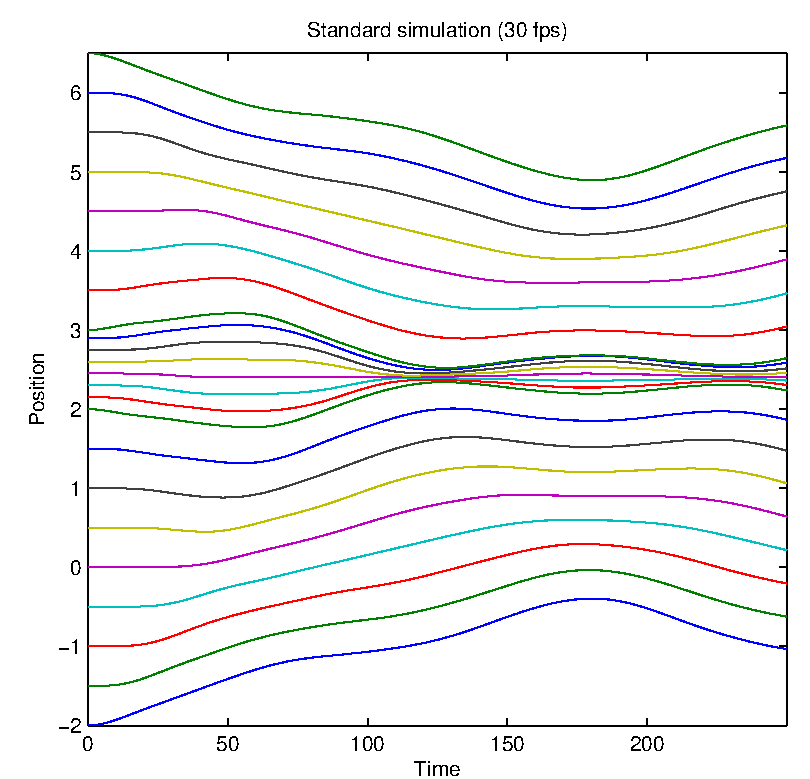
\includegraphics[width=\textwidth]{../images/standard_multiscale_30fps.pdf}
        \caption{30 fps}
        \label{fig:std_multi_30fps}
    \end{subfigure}
    \begin{subfigure}[t]{0.5\textwidth}
        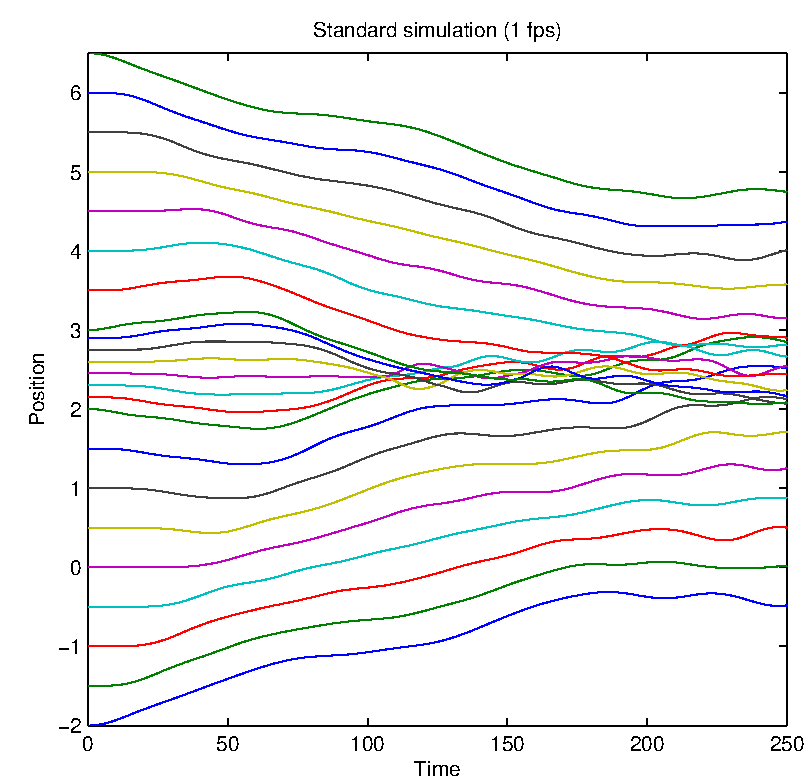
\includegraphics[width=\textwidth]{../images/standard_multiscale_1fps.pdf}
        \caption{1 fps}
        \label{fig:std_multi_1fps}
    \end{subfigure}
    \caption{Standard simulations of particles distributed with two scales using
    different timestep sizes}
    \label{fig:std}
\end{figure}

\subsection{Adapt-on-switch}
\label{sec:experiment_switch}
As mentioned in section \ref{sec:method_switch} the Adapt-on-switch method
can be implemented using either a relative or a absolute adaption of the
timestep. In our experiments we have tested out both methods defining the
relative adaption to scale the timestep by a factor of $\frac{1}{100}$ and
the absolute solution to set the timestep to $\frac{1}{30}$ when switches are
detected since this generated nice simulations for the standard simulation.
Furthermore the up-scaling for the relative scheme is set to a factor of 10
since we wish to avoid running into new switches immediately.

Figure \ref{fig:switch} shows the result of running the multi-scale
simulation at 1 fps using the Adapt-on-switch scheme, where the
red crosses mark timesteps at which a switch is predicted in the
following step and hence the schemes are ``activated''. Figure
\ref{fig:switch_multi_1fps_relative} is simulated using the relative scheme
and figure \ref{fig:switch_multi_1fps_absolute} is simulated using the
absolute scheme. As we clearly see in both figures the schemes fail to correct
the simulations in spite of the switch prediction. Once the first switch of
each of the simulations occurs the simulations will change behavior and hence
the first red cross marks the point at which the simulation can be rejected
from being correct.

Taking these observations into account we can safely say that the
Adapt-on-switch method/scheme is not working for our multi-scale simulation. This does
however not mean that the method couldn't work for other domains or other
refinements of the method. The problem with the scheme is that the prediction
of switches is done too late in the simulation. Once we detect the switches
it is too late to do anything about them given our model of the mass-spring
system. In order for the scheme to work properly it should be modified to be
able to perform the detection of switches earlier in the simulation if such a
prediction can be made reliably.

In the real world the spring force would ``bend'' towards $\pm \infty$ once
the spring is stretched or contracted too much resulting in a maximum and
minimum spring length. In other words the linear model that we use does not
suffice when using the Adapt-on-switch scheme, since the spring forces aren't
reacting the way we need them to when a spring is contracted. Having used a
more realistic choice of model could possibly have had a positive impact of
the use of this scheme. This would cause the spring force of the spring
in question to grow in order to avoid the switch.

As a sidenote it should be mentioned that we very shortly tested out an
alternative way of calculating the adaptive stepsize to confirm the hypothesis
above. We predicted how long a timestep we could take before the switch would
occur and then divided this steplength by 2 to get a new timestep length. This
generated infeasibly small timesteps forcing us to stop the simulation before
the time limit $t_{stop}$ was reached. This supports our hypothesis of the
incompatibility between the domain and the Adapt-on-switch method in the current
state.

\begin{figure}[H]
    \begin{subfigure}[t]{0.5\textwidth}
        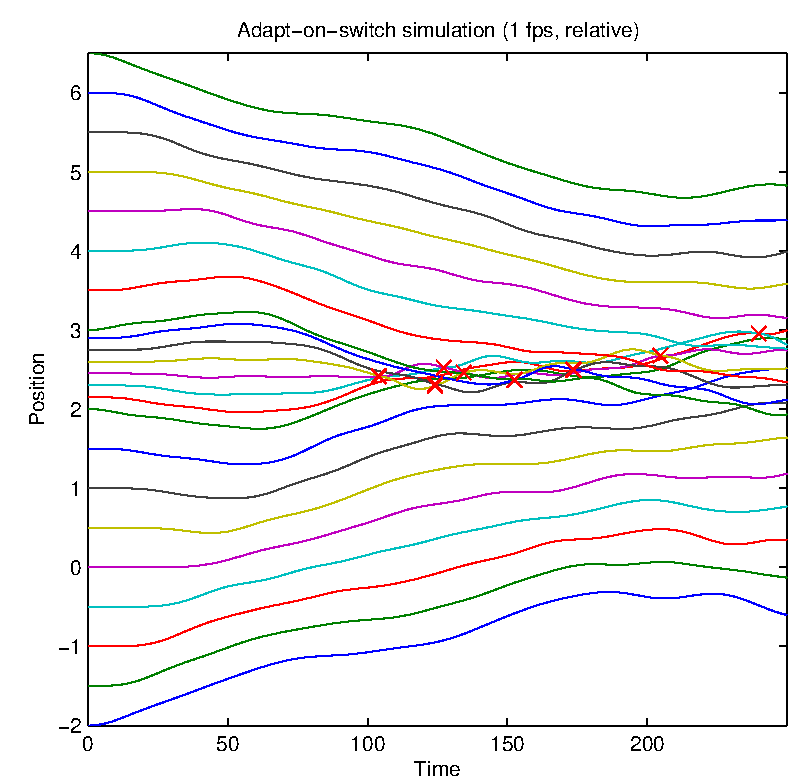
\includegraphics[width=\textwidth]{../images/switch_multiscale_1fps_relative.pdf}
        \caption{Relative timestepping ($\Delta t = \frac{\Delta t}{100}$)}
        \label{fig:switch_multi_1fps_relative}
    \end{subfigure}
    \begin{subfigure}[t]{0.5\textwidth}
        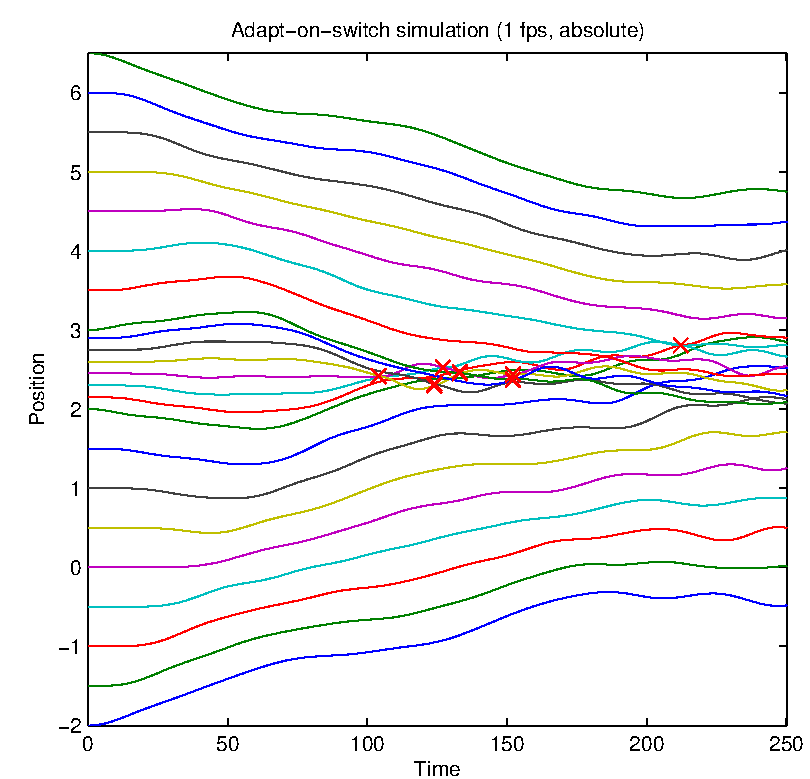
\includegraphics[width=\textwidth]{../images/switch_multiscale_1fps_absolute.pdf}
        \caption{Absolute timestepping ($\Delta t = \frac{1}{30}$)}
        \label{fig:switch_multi_1fps_absolute}
    \end{subfigure}
    \caption{Adapt-on-switch simulation of particles distributed with two
scales using 1 fps. The red crosses mark times at which the scheme predicts a
switch in the following iteration.}
    \label{fig:switch}
\end{figure}

\subsection{Atomic Updating using Heuristics}
\label{sec:experiments_atomic}
The AUH method concists of two heuristics for determining whether an element
should be updated or not: steps since last update $n_{last}$, and the ratio
$r_{last}$ between the spring length in last update and the current length.

We first test the method using only the first heuristic which will give us
synchronized updates of all vertices every $r_{last}$. step. Using the same
setup as the multi-scale simulation we perform simulations using the AUH method
with the length ratio heuristic ignored, the timestep set to $\Delta t =
\frac{1}{10}$ (10 fps) and varing $n_{last}$ across three different simulations.
Figure \ref{fig:atomic_multi_sbound} (\ref{fig:atomic_multi_10sbound} to
\ref{fig:atomic_multi_69sbound}) shows the resulting simulations where
figures \ref{fig:atomic_multi_10sbound}, \ref{fig:atomic_multi_68sbound},
and \ref{fig:atomic_multi_69sbound} uses a $n_{last}$ of 10, 68, and 69
respectively.

Simulating using 10 fps and $n_{last} = 10$ give us the same amount of
velocity updates as the standard simulation using 1 fps (which had switches).
Using the AUH scheme we do however get a nice and smooth simulation with no
problems. As can be seen in the figures \ref{fig:atomic_multi_68sbound} and
\ref{fig:atomic_multi_69sbound} we are able to perform the simulation using
$n_{last} = 68$ without having switches occuring whereas using $n_{last} =
69$ results in switches occuring. In other words we are able to perform the
simulation at 10 fps but with 6.8 seconds between acceleration and velocity
calculations. This is a result of combining the explicit Euler method with
the AUH scheme. The scheme extrapolates the position at the last
acceleration and velocity update to a position close in time to the next
update position. It then uses this position when updating the acceleration
and velocity again. Had we chosen an alternative time integration method this
advantage would most likely have been eliminated and let us perform the larger
timesteps with the standard simulation. This would however had increased the
computational cost of each timestep.

The second heuristic ($r_{last}$) should be activated when $r_{last}$ is
small. The bound $r_{b}$ for forcing updates based on $r_{last}$ should
however be defined according to the simulation in question. Likewise the
first heuristic should be activated in between the activation of the $r_b$
bound to force a minimum of updates between the endpoints of the spring
motion.

In order to test out the heuristic we first perform a simulation using
only 3 equally distributed particles at 10 fps for 250 seconds. The initial
state of the simulation is: timestep $\Delta t = 0.1$, damping $C_s = 0.01$,
stiffness $K_s = 0.5$, initial vertex positions 2, 0 and -2, and spring rest
length 1.6 for both springs. By performing a series of simulations we find
the most optimal combination of the two heuristics for the simulation to be
$r_{last} = 20$, $r_b = 1.002$. Figure \ref{fig:atomic_uniform} shows the
resulting simulation plots displaying positions as a function of the time
using the AUH method (\ref{fig:atomic_uniform_10fps_0}) and the standard
method (\ref{fig:atomic_uniform_10fps_1}). The green dots of the AUH plot
shows the update positions.

As we see from the AUH plot, the heuristics start out by updating the
accelerations and velocities at the endpoints of the spring motions as
intended. Likewise the stepping bound activates updates at lower frequency
(every 20th step) in between the endpoints as intended. When time passes the
system is being dampened too much compared to the small damping factor. At the
end of the simulation the $r_b$ bound activates updates in all steps of the
simulation. When we compare the resulting simulation of the AUH and standard
methods we are observing quite large differences. As mentioned the AUH method
dampens the system too much when the $r_b$ bound is not activated, and hence we
get the observed difference in simulation result.

Figure \ref{fig:atomic_multi_both} shows the resulting simulation plot
using the AUH method and setting $n_{last} = 10,~r_b = 1.01$ for the
multi-scale simulation. As for the previous simulation example we have
estimated the best values of $n_{last}$ and $r_b$ by varying both and
inspecting the resulting simulation. A switch occurs at time $t = 104$ which
corrupts and invalidates the rest of the simulation.

The conclusion of the application of this method is, that the first heuristic
was very succesful in case we need to use the explicit Euler method. The second
heuristic was however only affecting the outcome of the simulations negatively,
and thus it should be rejected.

\begin{figure}[H]
    \begin{subfigure}[t]{0.5\textwidth}
        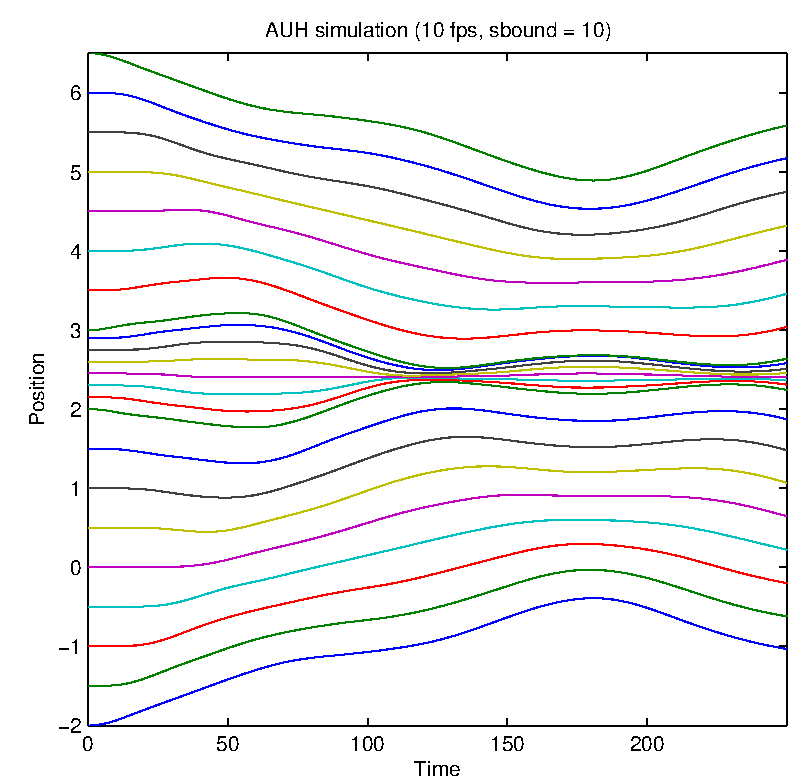
\includegraphics[width=\textwidth]{../images/atomic_multiscale_10fps_10sbound.pdf}
        \caption{$n_{last} = 10$, $r_{last}$ ignored}
        \label{fig:atomic_multi_10sbound}
    \end{subfigure}
    \begin{subfigure}[t]{0.5\textwidth}
        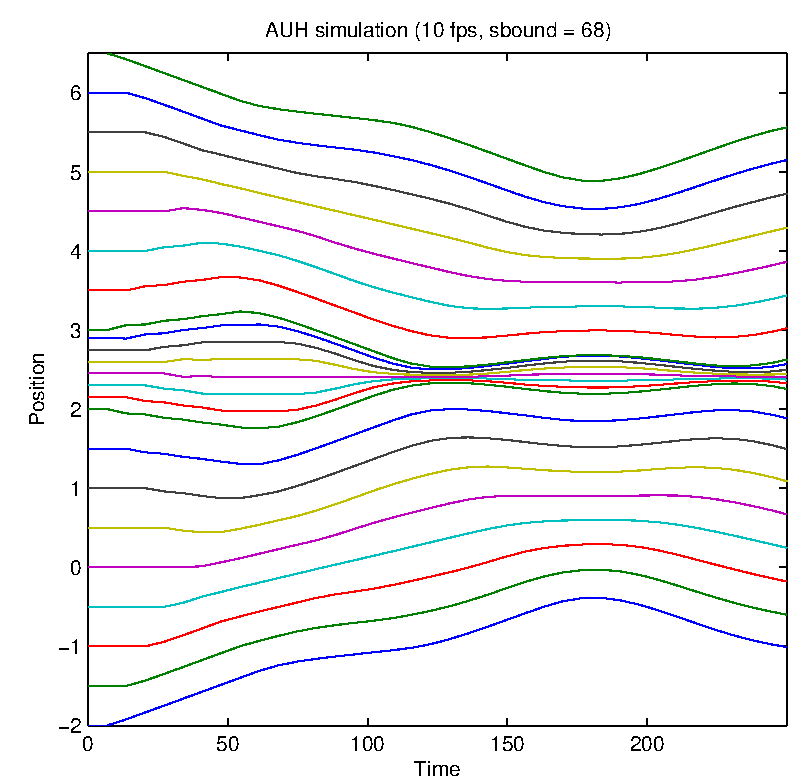
\includegraphics[width=\textwidth]{../images/atomic_multiscale_10fps_68sbound.pdf}
        \caption{$n_{last} = 68$, $r_{last}$ ignored}
        \label{fig:atomic_multi_68sbound}
    \end{subfigure}
    \begin{subfigure}[t]{0.5\textwidth}
        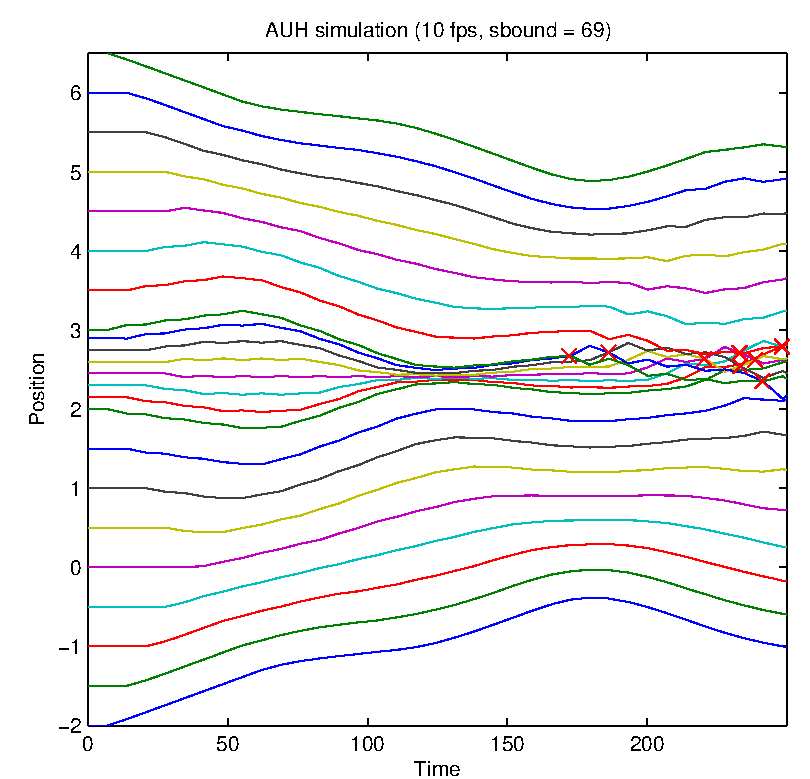
\includegraphics[width=\textwidth]{../images/atomic_multiscale_10fps_69sbound.pdf}
        \caption{$n_{last} = 69$, $r_{last}$ ignored}
        \label{fig:atomic_multi_69sbound}
    \end{subfigure}
    \begin{subfigure}[t]{0.5\textwidth}
        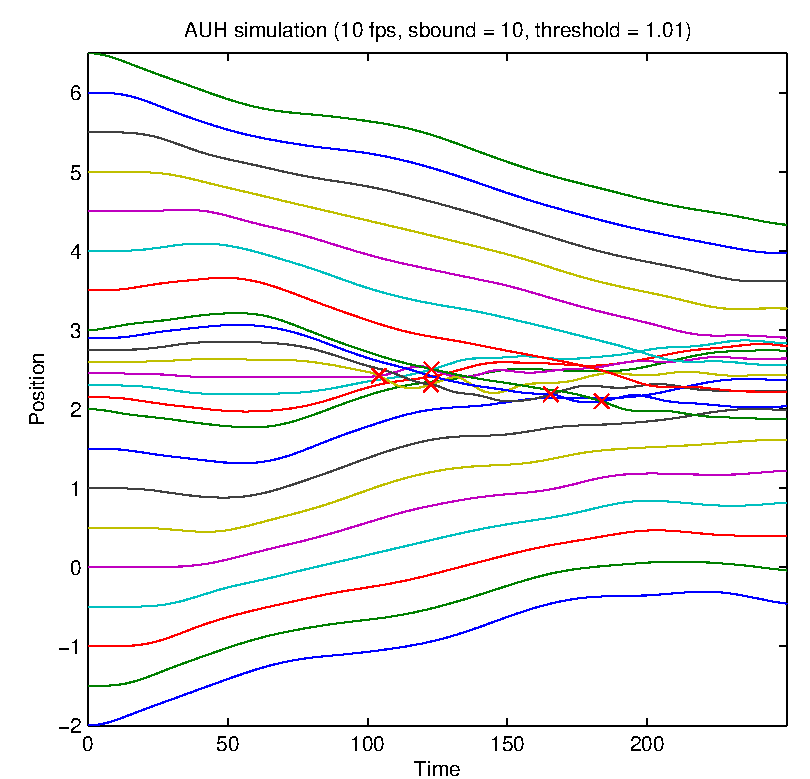
\includegraphics[width=\textwidth]{../images/atomic_multiscale_10fps_both.pdf}
        \caption{$n_{last} = 10, r_{b} = 1.01$}
        \label{fig:atomic_multi_both}
    \end{subfigure}
    \caption{Simulations using the AUH method at 10 fps with various number of
    steps since last update.}
    \label{fig:atomic_multi_sbound}
\end{figure}

\begin{figure}
    \begin{subfigure}[t]{0.5\textwidth}
        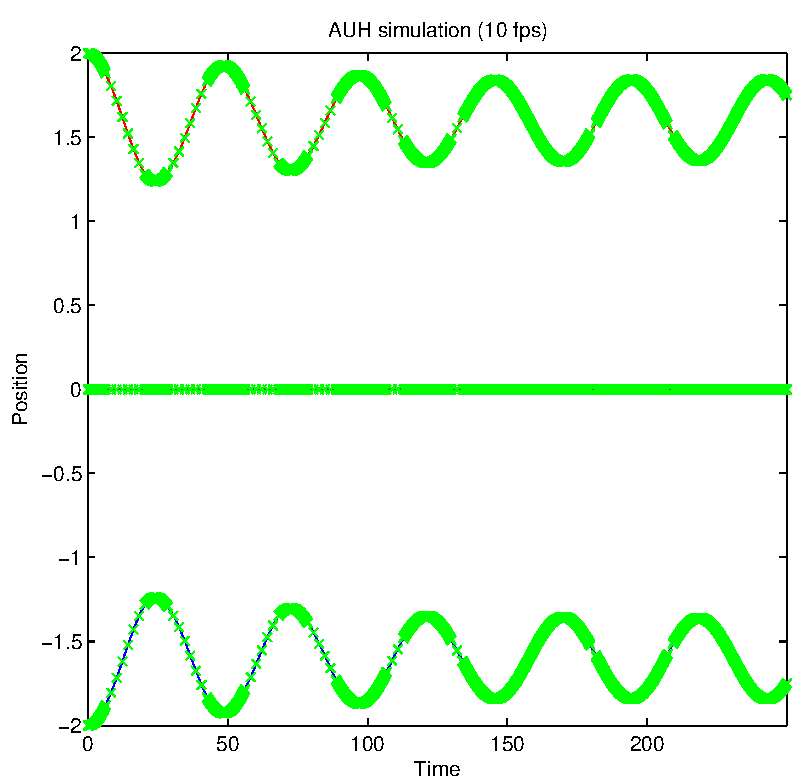
\includegraphics[width=\textwidth]{../images/atomic_uniform_10fps_0.pdf}
        \caption{AUH method ($r_b = 1.002,~r_{last} = 20$)}
        \label{fig:atomic_uniform_10fps_0}
    \end{subfigure}
    \begin{subfigure}[t]{0.5\textwidth}
        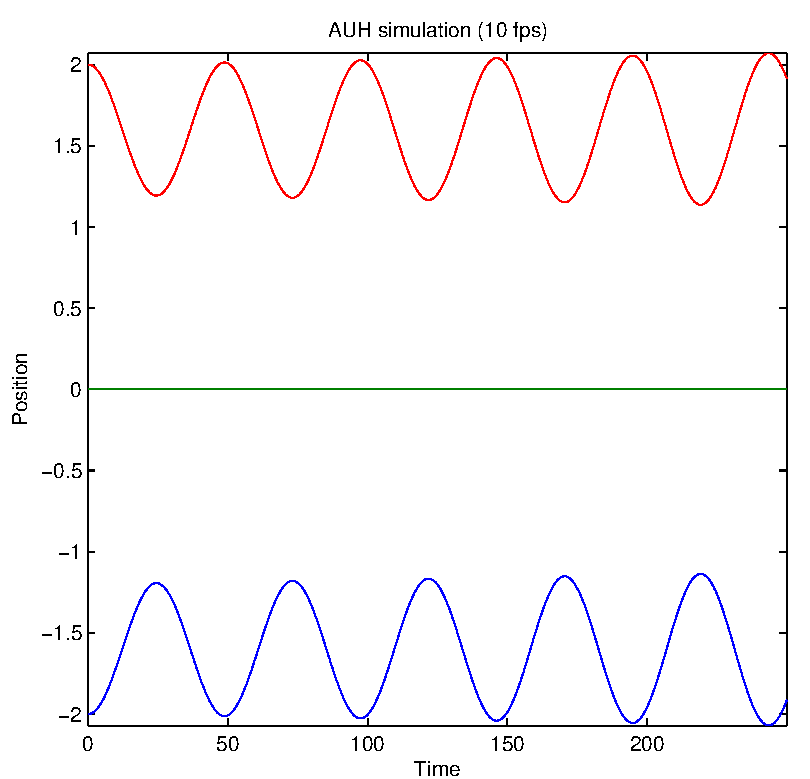
\includegraphics[width=\textwidth]{../images/atomic_uniform_10fps_1.pdf}
        \caption{Standard method}
        \label{fig:atomic_uniform_10fps_1}
    \end{subfigure}
    \caption{Simple 3-vertex simulations at 10 fps}
    \label{fig:atomic_uniform}
\end{figure}

\subsection{Global Estimated Acceleration}
\label{sec:experiments_inverse}
In the GEA method we perform adaption of the timestep according to equation
\ref{eq:inverse}. We therefore first wish to explore what this adaption
means for a simple simulation, before exploring the effect on the particle
system used in the previous method experiments. We use the following
constants: $C_s = 0.5$, $K_s = 0.3$, $l_{0,s} = 1.6$, and the initial vertex
positions are 2, 0, and -2. Furthermore given our simulation we define our
timestep to $\Delta t_{GEA} = \Delta t^{0.8}\cdot \frac{1}{250}$ using
the definition of $\Delta t$ in equation \ref{eq:inverse} in order to get
steps of proper size. Figure \ref{fig:inverse_uniform_30fps_0} shows the
resulting simulation displaying the position as a function of the time.
The red lines show a standard simulation at 5 fps, the black lines show a
standard simulation at 2.5 fps, and the blue lines show the GEA simulation.
We observe that the three simulations are coinciding and hence our adaption of
the timestep has no negative impact of the simulation outcome. Looking at figure
\ref{fig:inverse_uniform_30fps_steps} we see the timestep sizes during the
simulations displayed with the same colors as the simulation figure. We see
that the GEA simulation varies it's timestep in between the two standard
simulation timesteps and hence in this simulation the varying timestep isn't
really beneficial as a standard simulation with lower fps is sufficient and
hence less costly.

We now compare the GEA and standard simulation methods using the same
multi-scale simulation setup. Here we have defined the varying timestep
as $\Delta t_{GEA} = \Delta t^{0.8} \cdot \frac{1}{120}-0.038$ again
using the definition of $\Delta t$ in equation \ref{eq:inverse}.
Figure \ref{fig:inverse_multiscale} shows resulting plots of the
timestep size as a function of the time of the simulation (figure
\ref{fig:inverse_multiscale_steps}), and the accumulated number
of timesteps as a function of the time of the simulation (figure
\ref{fig:inverse_multiscale_cumstep}). The blue lines are the results for
the GEA method and the red lines are the results for the standard method
simulated at 1.8 fps, which is the lowest fps at which no switches occur.
Looking solely at the simulation-part of the previous methods (the first 250
seconds) the GEA simulation used 455 steps while the standard simulation
used 451 steps. If we however let the simulation run for a longer period
of time, the GEA method surpasses the standard simulation. As we see in
figure \ref{fig:inverse_multiscale_cumstep} the difference in accumulated
number of timesteps rises as time passes. 20,000 seconds into the
simulation the standard simulation has used 36001 steps and GEA has used
30145 steps. This is caused by the dampening of the system. As the acceleration
of the springs decreases, the timesteps rise as can be seen in figure
\ref{fig:inverse_uniform_30fps_steps} and \ref{fig:inverse_multiscale_steps}.
By carefully scaling the timestep varying heuristic, the timestep adaption
gains benefit over the standard simulation. The downside is however, that we
first have to put an effort into scaling the heuristic to fit our simulation,
but for the standard simulation we likewise have to experiment with the
timestep size in order to find the threshold at which switches start occuring.

Looking at the execution time the GEA method takes around 4.6 seconds and the
standard simulation takes around 3.7 seconds to simulate 20,000 seconds at my
personal laptop (2.53 GHz dualcore, 4GB memory) using my current Matlab 2013b
implementation. This shows that the overhead of computing the heuristic and
modifying the timestep for the GEA method in the current setup and simulation
is more expensive than simply performing the standard simulation. In short we
have gained no advantage. The execution time for the GEA method could however
possibly be optimized and decreased using another programming language.
Furthermore the advantage of the adapting is dependent of the simulation in
question. Further investigation of the possible use of the GEA method
should therefore be performed before a final conclusion can be made.

Another heuristic which potentially could be used for the adaptive
timestepping would be the acceleration (as opposed to the inverse of the
acceleration in equation \ref{eq:inverse}). This could be done by having a
basis timestep which is sufficient when the springs have a low acceleration.
When the acceleration rises the timestep is decreased in stages instead
of a direct one-to-one mapping depending on the order of magnitude of the
acceleration.

\begin{figure}
    \begin{subfigure}[t]{0.5\textwidth}
        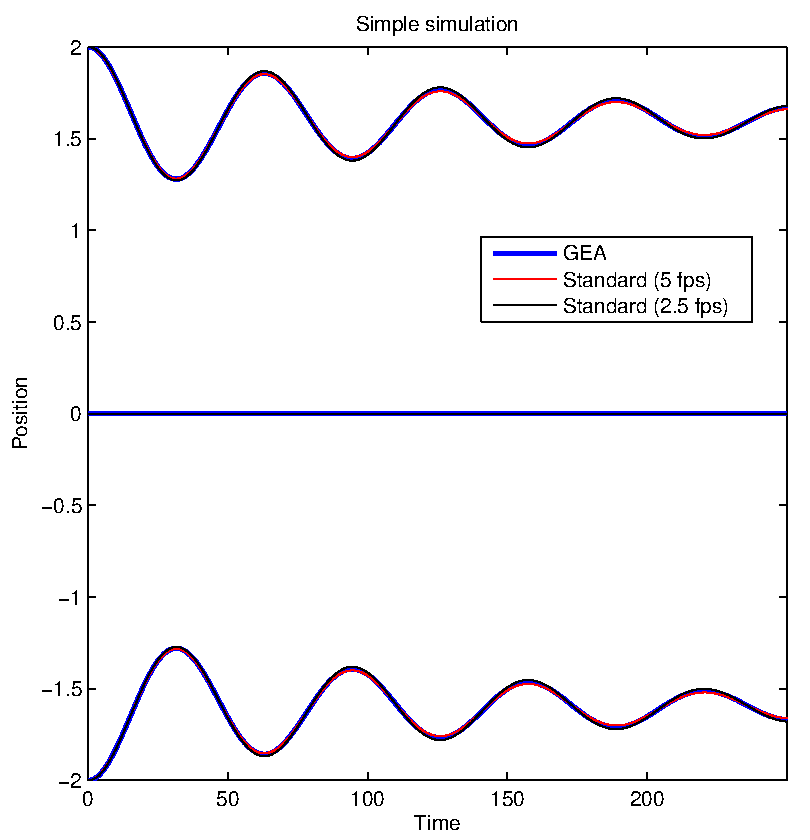
\includegraphics[width=\textwidth]{../images/inverse_uniform_30fps.pdf}
        \caption{Simulation using GEA (blue) and standard (red) simulation methods with
        position as a function of the time of the simulation.}
        \label{fig:inverse_uniform_30fps_0}
    \end{subfigure}
    \begin{subfigure}[t]{0.5\textwidth}
        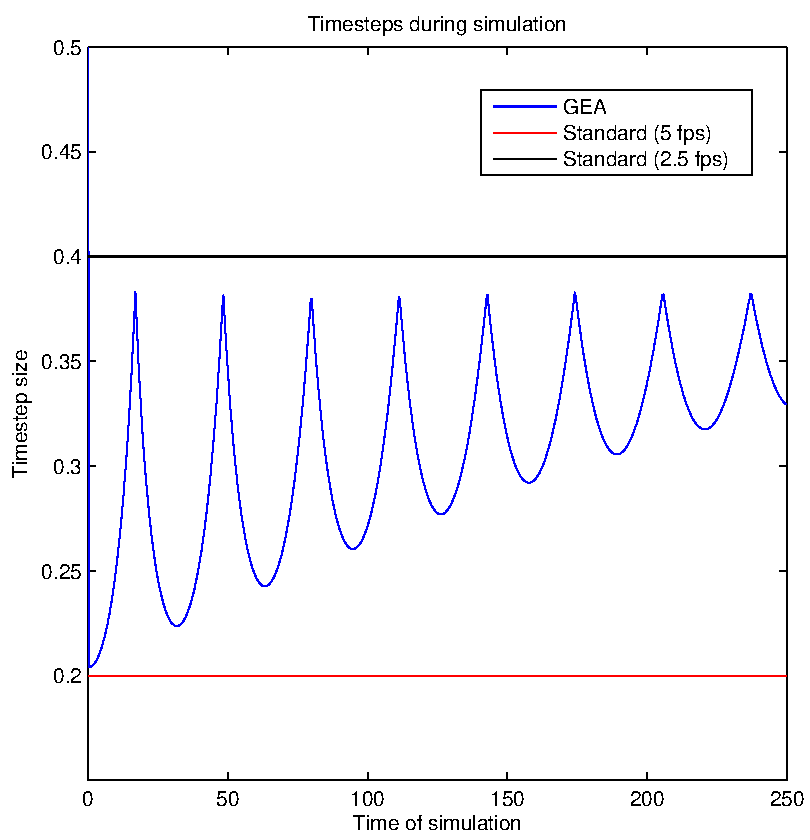
\includegraphics[width=\textwidth]{../images/inverse_uniform_30fps_steps.pdf}
        \caption{Timestep size for GEA (blue) and standard (red) of the simulation in
            \ref{fig:inverse_uniform_30fps_0}}
        \label{fig:inverse_uniform_30fps_steps}
    \end{subfigure}
    \caption{GEA compared with standard simulation on simple 3-vertex
    mass-spring system}
    \label{fig:inverse}
\end{figure}
\begin{figure}
    \begin{subfigure}[t]{0.5\textwidth}
        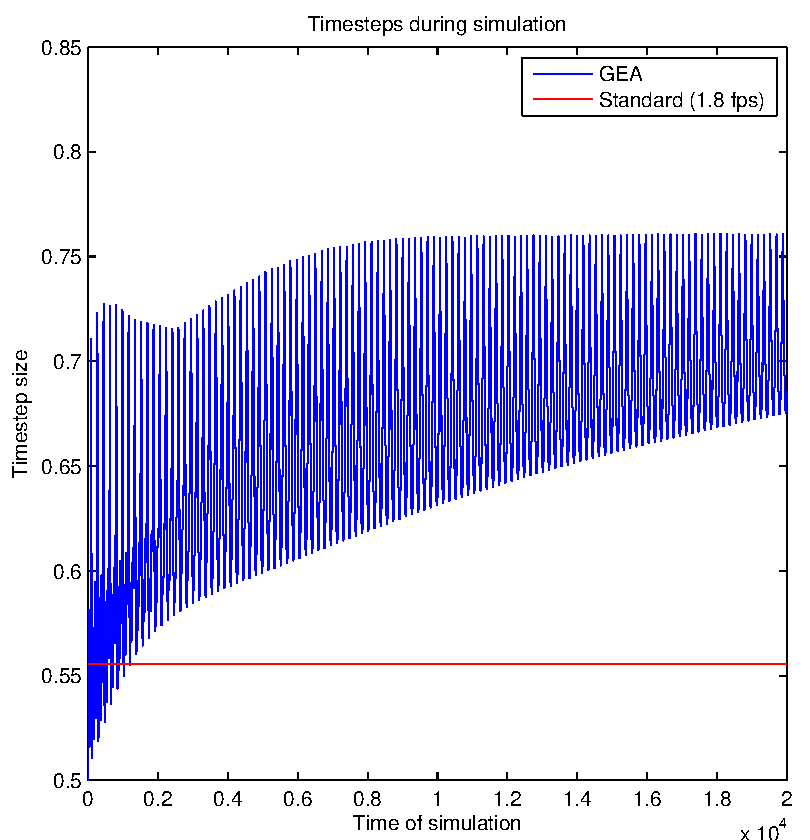
\includegraphics[width=\textwidth]{../images/inverse_multiscale_steps.pdf}
        \caption{Timestep size for GEA (blue) and standard (red) as a function
        of the time passed}
        \label{fig:inverse_multiscale_steps}
    \end{subfigure}
    \begin{subfigure}[t]{0.5\textwidth}
        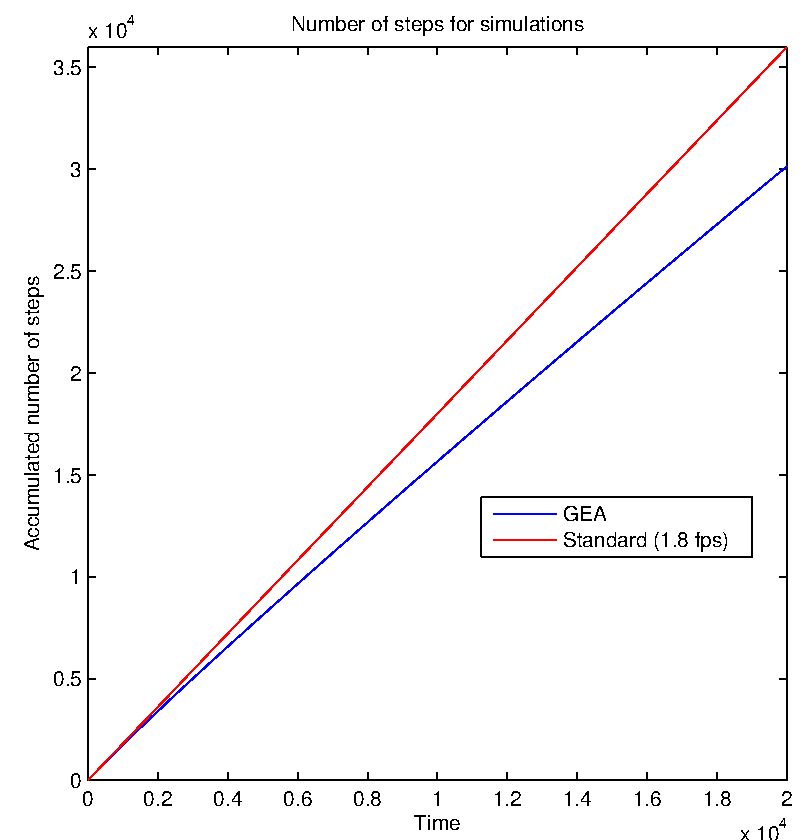
\includegraphics[width=\textwidth]{../images/inverse_multiscale_cumstep.pdf}
        \caption{Accumulated number of steps taken as a function of the time passed for GEA
        (blue) and standard (red)}
        \label{fig:inverse_multiscale_cumstep}
    \end{subfigure}
    \caption{GEA compared with standard simulation on particles distributed with
        two scales simulated for 20,000 seconds}
    \label{fig:inverse_multiscale}
\end{figure}

%Examples of
%
%\begin{table}[H]
%\caption{Example table}
%\centering
%\begin{tabular}{llr}
%\toprule
%\multicolumn{2}{c}{Name} \\
%\cmidrule(r){1-2}
%First name & Last Name & Grade \\
%\midrule
%John & Doe & $7.5$ \\
%Richard & Miles & $2$ \\
%\bottomrule
%\end{tabular}
%\end{table}

%------------------------------------------------

\section{Further discussion and future work}
\label{sec:future_work}
We here present a short discussion of the methods with the purpose of presenting
possible future work.

All three methods proposed in this paper could possibly benefit from being
tested using alternative integration methods. This is due to the fact that
the explicit Euler method is quite numerically unstable if too large steps
are taken. Using a more stable integration method could therefore potentially
change the outcome of the experiments of the methods.

As mentioned in section \ref{sec:experiment_switch} the Adapt-on-switch method
could possibly be succesful on a domain modelling the behavior of springs more
naturally and hence future work could be done in this direction.

The GEA method should be further investigated to see if it could
give a computational benefit or not as concluded in section
\ref{sec:experiments_inverse}. Likewise the alternative acceleration heuristic
proposed at the end of section \ref{sec:experiments_inverse} could potentially
be implemented, tested and compared to the inverse acceleration heuristic of
the GEA method to see which of the two methods performs best.

As we saw in section \ref{sec:experiments} both the AUH method with the
$n_{last}$ heuristic (only) and the GEA method where (partially) succesful.
These methods and their applications should therefore be further investigated.
Combinations of these methods and heuristics could likewise be investigated in
order to get possibly faster LAOT schemes than the ones proposed, tested and
discussed in this report. An example of such a LAOT scheme could be a fully
atomic timestepping scheme where the inverse acceleration heuristic would be
applied to the atomic updating method. This would result in a LAOT method
which is both spatial and time adative. It would however require quite a lot
of bookkeeping and investigation of asynchronous update behavior, which is not
covered in this report due to the fact that the heuristic for the asynchronous
behaviour of the AUH method was rejected prior due to other flaws.

Finally the succesful schemes should be applied to hyperelastic material
simulations, which is the original motivation for the work of this report.

%------------------------------------------------

\section{Conclusion}
In this report we have described a 1-dimensional mass-spring system using the
explicit Euler. Furthermore we have proposed, described, tested and discussed
the three LAOT methods Adapt-on-switch, Atomic Updating using Heuristics, and
Global Estimated Acceleration and the heuristics for each of the methods.
All these methods (including the standard simulation) and heuristics were
implemented as described in this report.

The Adapt-on-switch method to predict and correct for spring switches was
rejected for this domain after testing. The AUH heuristic of using $r_{last}$
to perform asynchronious Atomic Updating of Accelerations was likewise
rejected after testing.

The AUH method using only the $n_{last}$ heuristic bound was succesful when
using the explicit Euler integration, but the advantage of the method is
likely to disappear when using other integration schemes.

The GEA method was succesful in increasing the timestep size over time and
hence decrease the number of total steps. It was however too computationally
heavy in the current implementation and should therefore be investigated further
before making a final conclusion.

Further future work was proposed for all three methods including amongst
others: testing all methods by using alternative integration schemes,
experimenting with combinations of the AUH and GEA methods and heuristics,
and applying the LAOT methods and heuristics for hyperelastic material
simulations.

%----------------------------------------------------------------------------------------
%	REFERENCE LIST
%----------------------------------------------------------------------------------------


\bibliography{bibliography}
\bibliographystyle{plain}

%----------------------------------------------------------------------------------------


\end{document}
